\section{Algorithm}\label{sec:optimization}


Assuming every face in the carton model is rigid, which means the interior angle in each plane stays the same. But planes can be bent during folding. \cxj{For example, a rigid plane can be bent during folding?}
%
Furthermore, planes are connected by hinges at the boundary of patches, and the planar layout has its front and back.

\subsection{Initialization}\label{sec:initialization}
In this section we explain the reason why using a specific angle to each fold edge, and constructing our initialized model. The basic idea is to interpret the folded state of a box as a series of rotation angles along each edge, where the problem of predicting the folded state is turned into a problem of predicting these angles.

Observe from existing data, two common rules are summarized as our basic idea of initialization.

\noindent
\textbf{Plane perpendicularity} The adjacent planes should not be paralleled, and we encourage them to be perpendicular. The term used here is
\begin{equation}
\alpha_{pe} = \sum_{i = 1}^{n} [\sin^{-1}(\mathbf{n}_1 \cdot \mathbf{n}_2)]^{2},
\label{equ:perp}
\end{equation}
where $\hat{n}_1$ and $\hat{n}_2$ denotes all possible combinations of normals of adjacent planes, and $n$ is the number of such combinations.

\noindent
\textbf{Plane parallelism} It was observed that two planes with same shape are probably paralleled, so we encourage more planes with same shape to be paralleled. The term is
\begin{equation}
\alpha_{pa} = \sum_{i = 1}^{n} [\cos^{-1}(\mathbf{n}_1 \cdot \mathbf{n}_2)]^{2},
\label{equ:para}
\end{equation}
where $\hat{n}_1$ and $\hat{n}_2$ denotes all possible combinations of normals of disadjacent planes that have same shape,  and $n$ is the number of such combinations.

By implementing the CMA-ES(Covariance Matrix Adaptation Evolution Strategy)~\cite{CMAES} adding the above two constrains, the initialization result is shown in Figure~\ref{fig:initial}. Note that as the input variables are fold angles of edges, $\mathbf{n}_1 \cdot \mathbf{n}_2$ is represented by $cos\alpha$ where $\alpha$ is the angle between these two normal vectors. 

We can see from the five examples shown in Figure~\ref{fig:initial}, the up three examples can have ideal results and the bottom two results are even not closed at last, which actually caused by the two constrains above lead to a result that each angle of each edge is always $\pi/2$. As a consequence, some irregular boxes will present a boxy shape which will be refined later by user interaction.

As for our initialization, $\pi/2$ is finally set to each angle and this causes more than half of boxes folded correctly in our database.


\cxj{do not use angle. do you use parallelism?}
%\begin{figure}
%	\centering
%	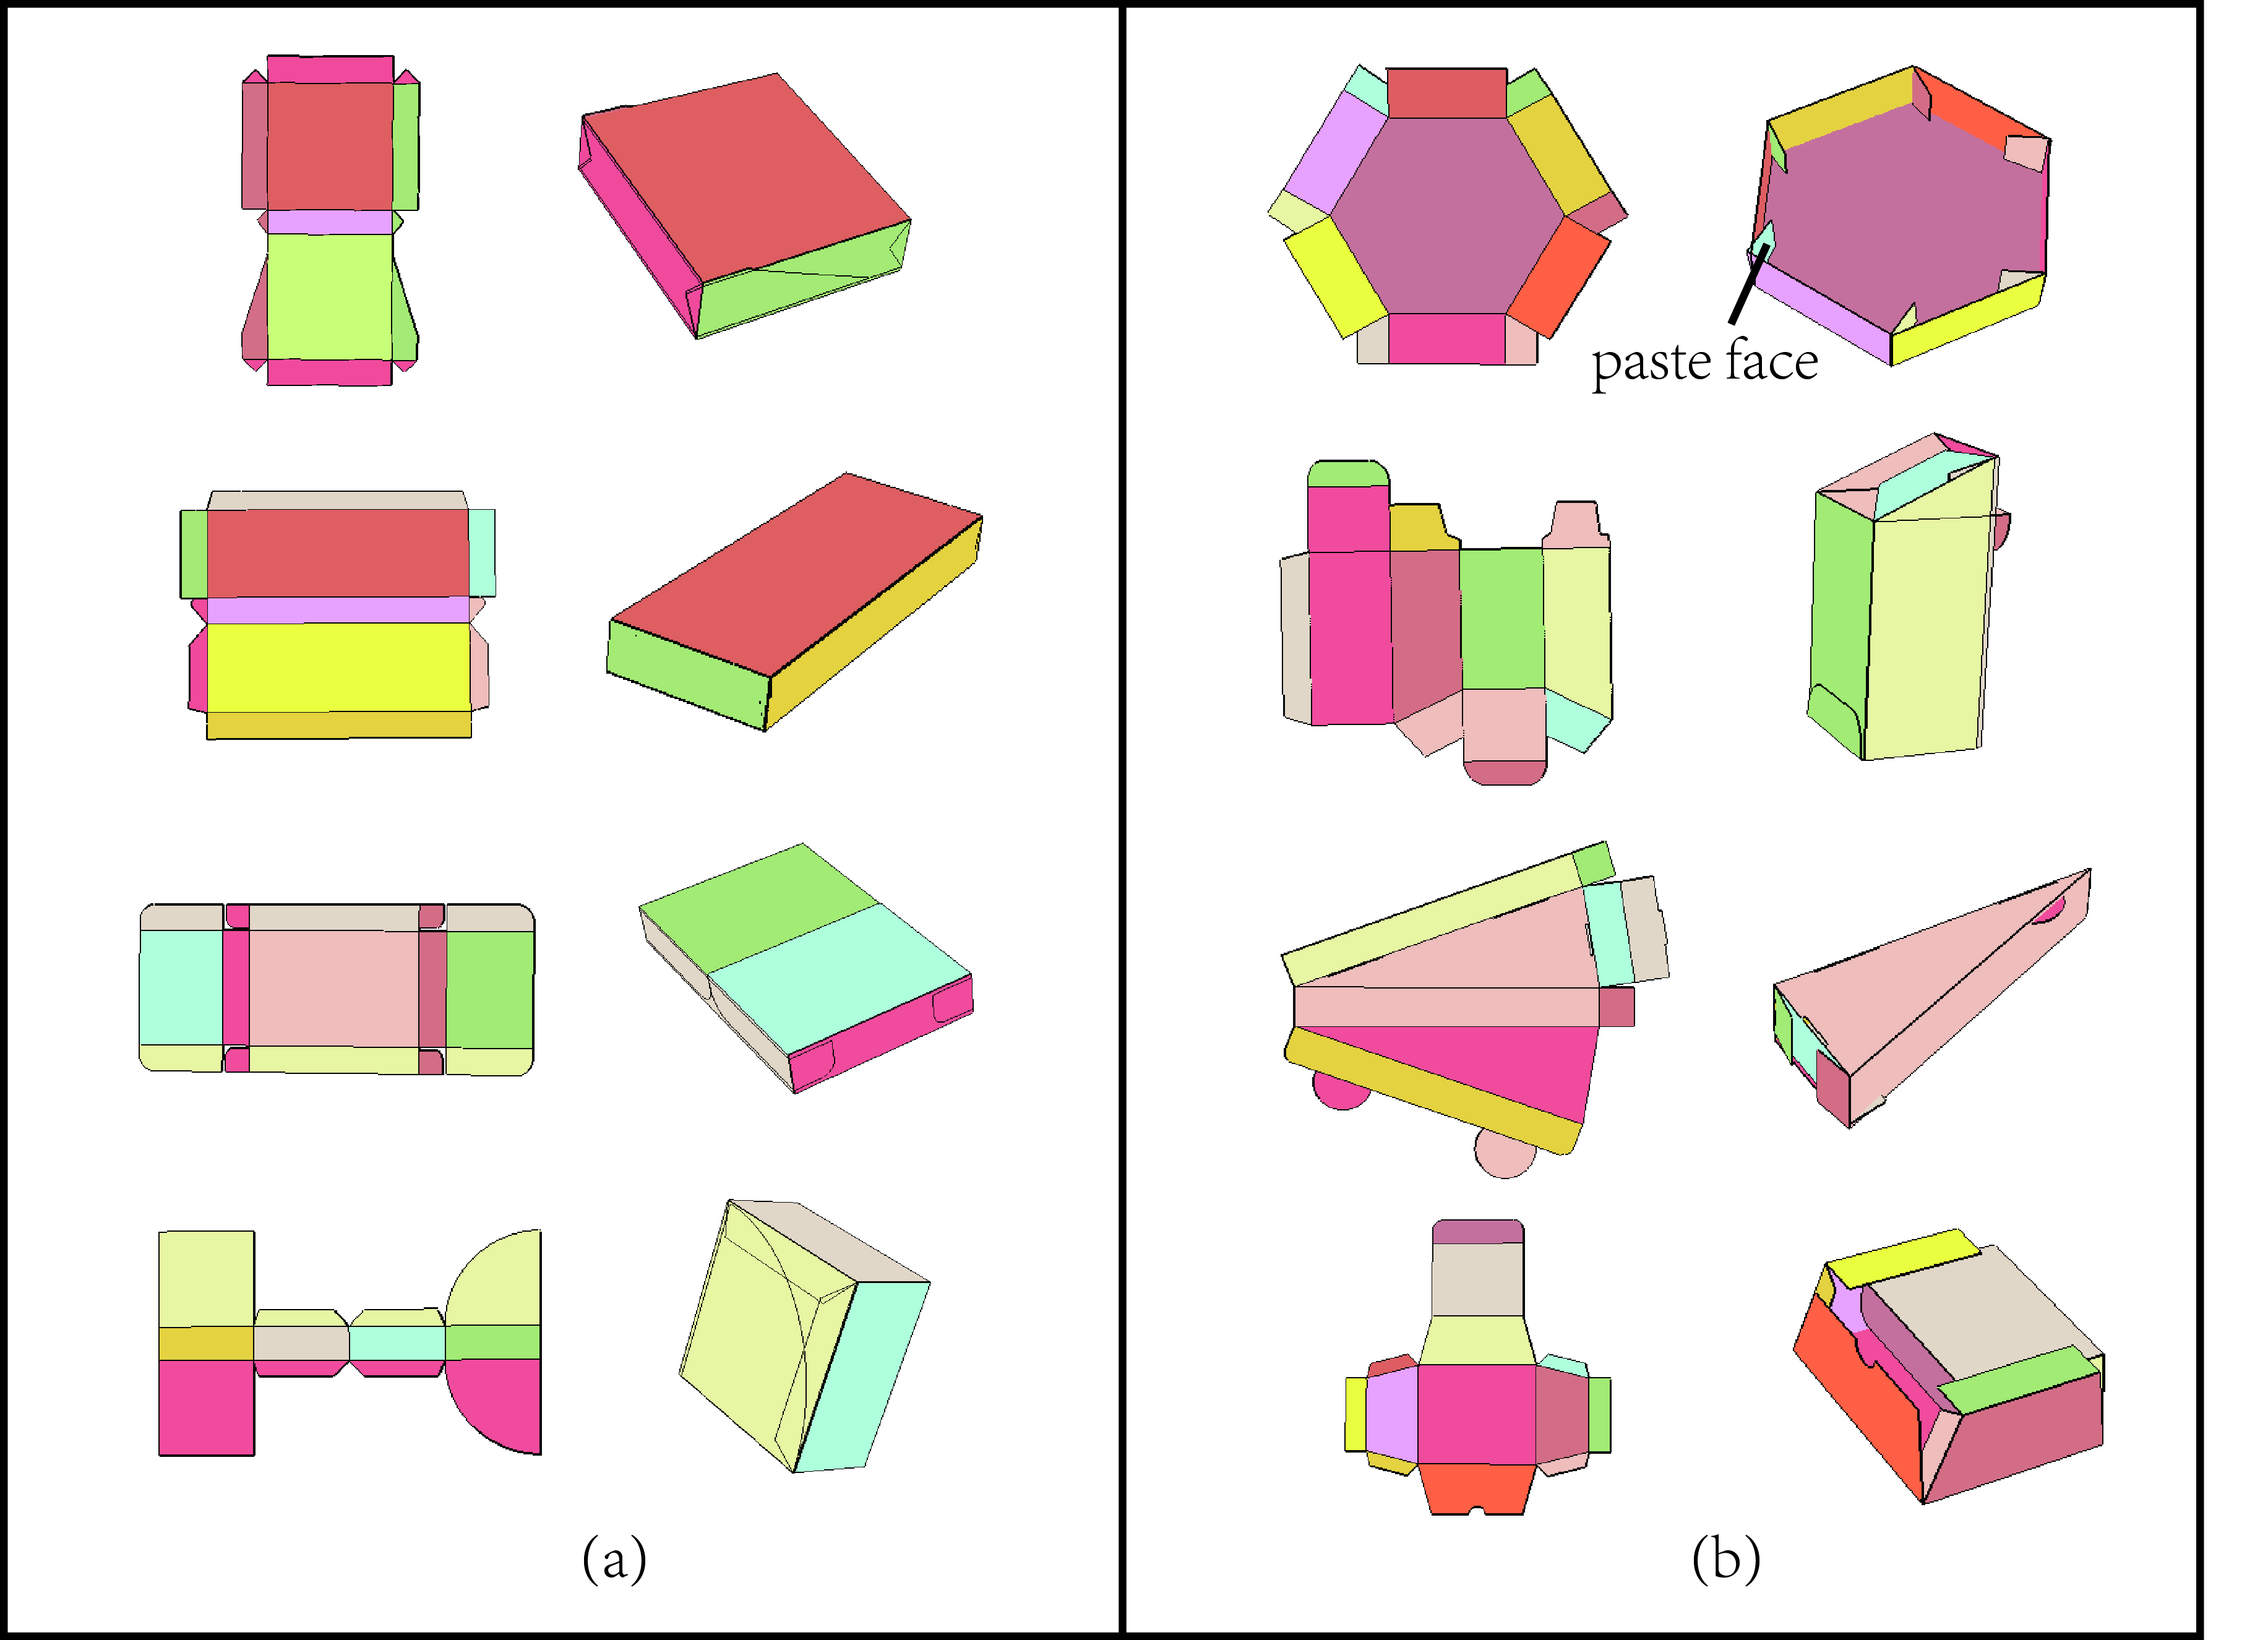
\includegraphics[width=0.9\textwidth]{images/initial.jpg}
%	\caption{Initialized results of five examples. Each row is an example, and the first column is the 2D design layout, the second column is the polymesh created from layout, the third column is the initialized results optimized with the two constrains.}
%	\label{fig:initial}
%\end{figure}

\begin{figure}
	\centering
	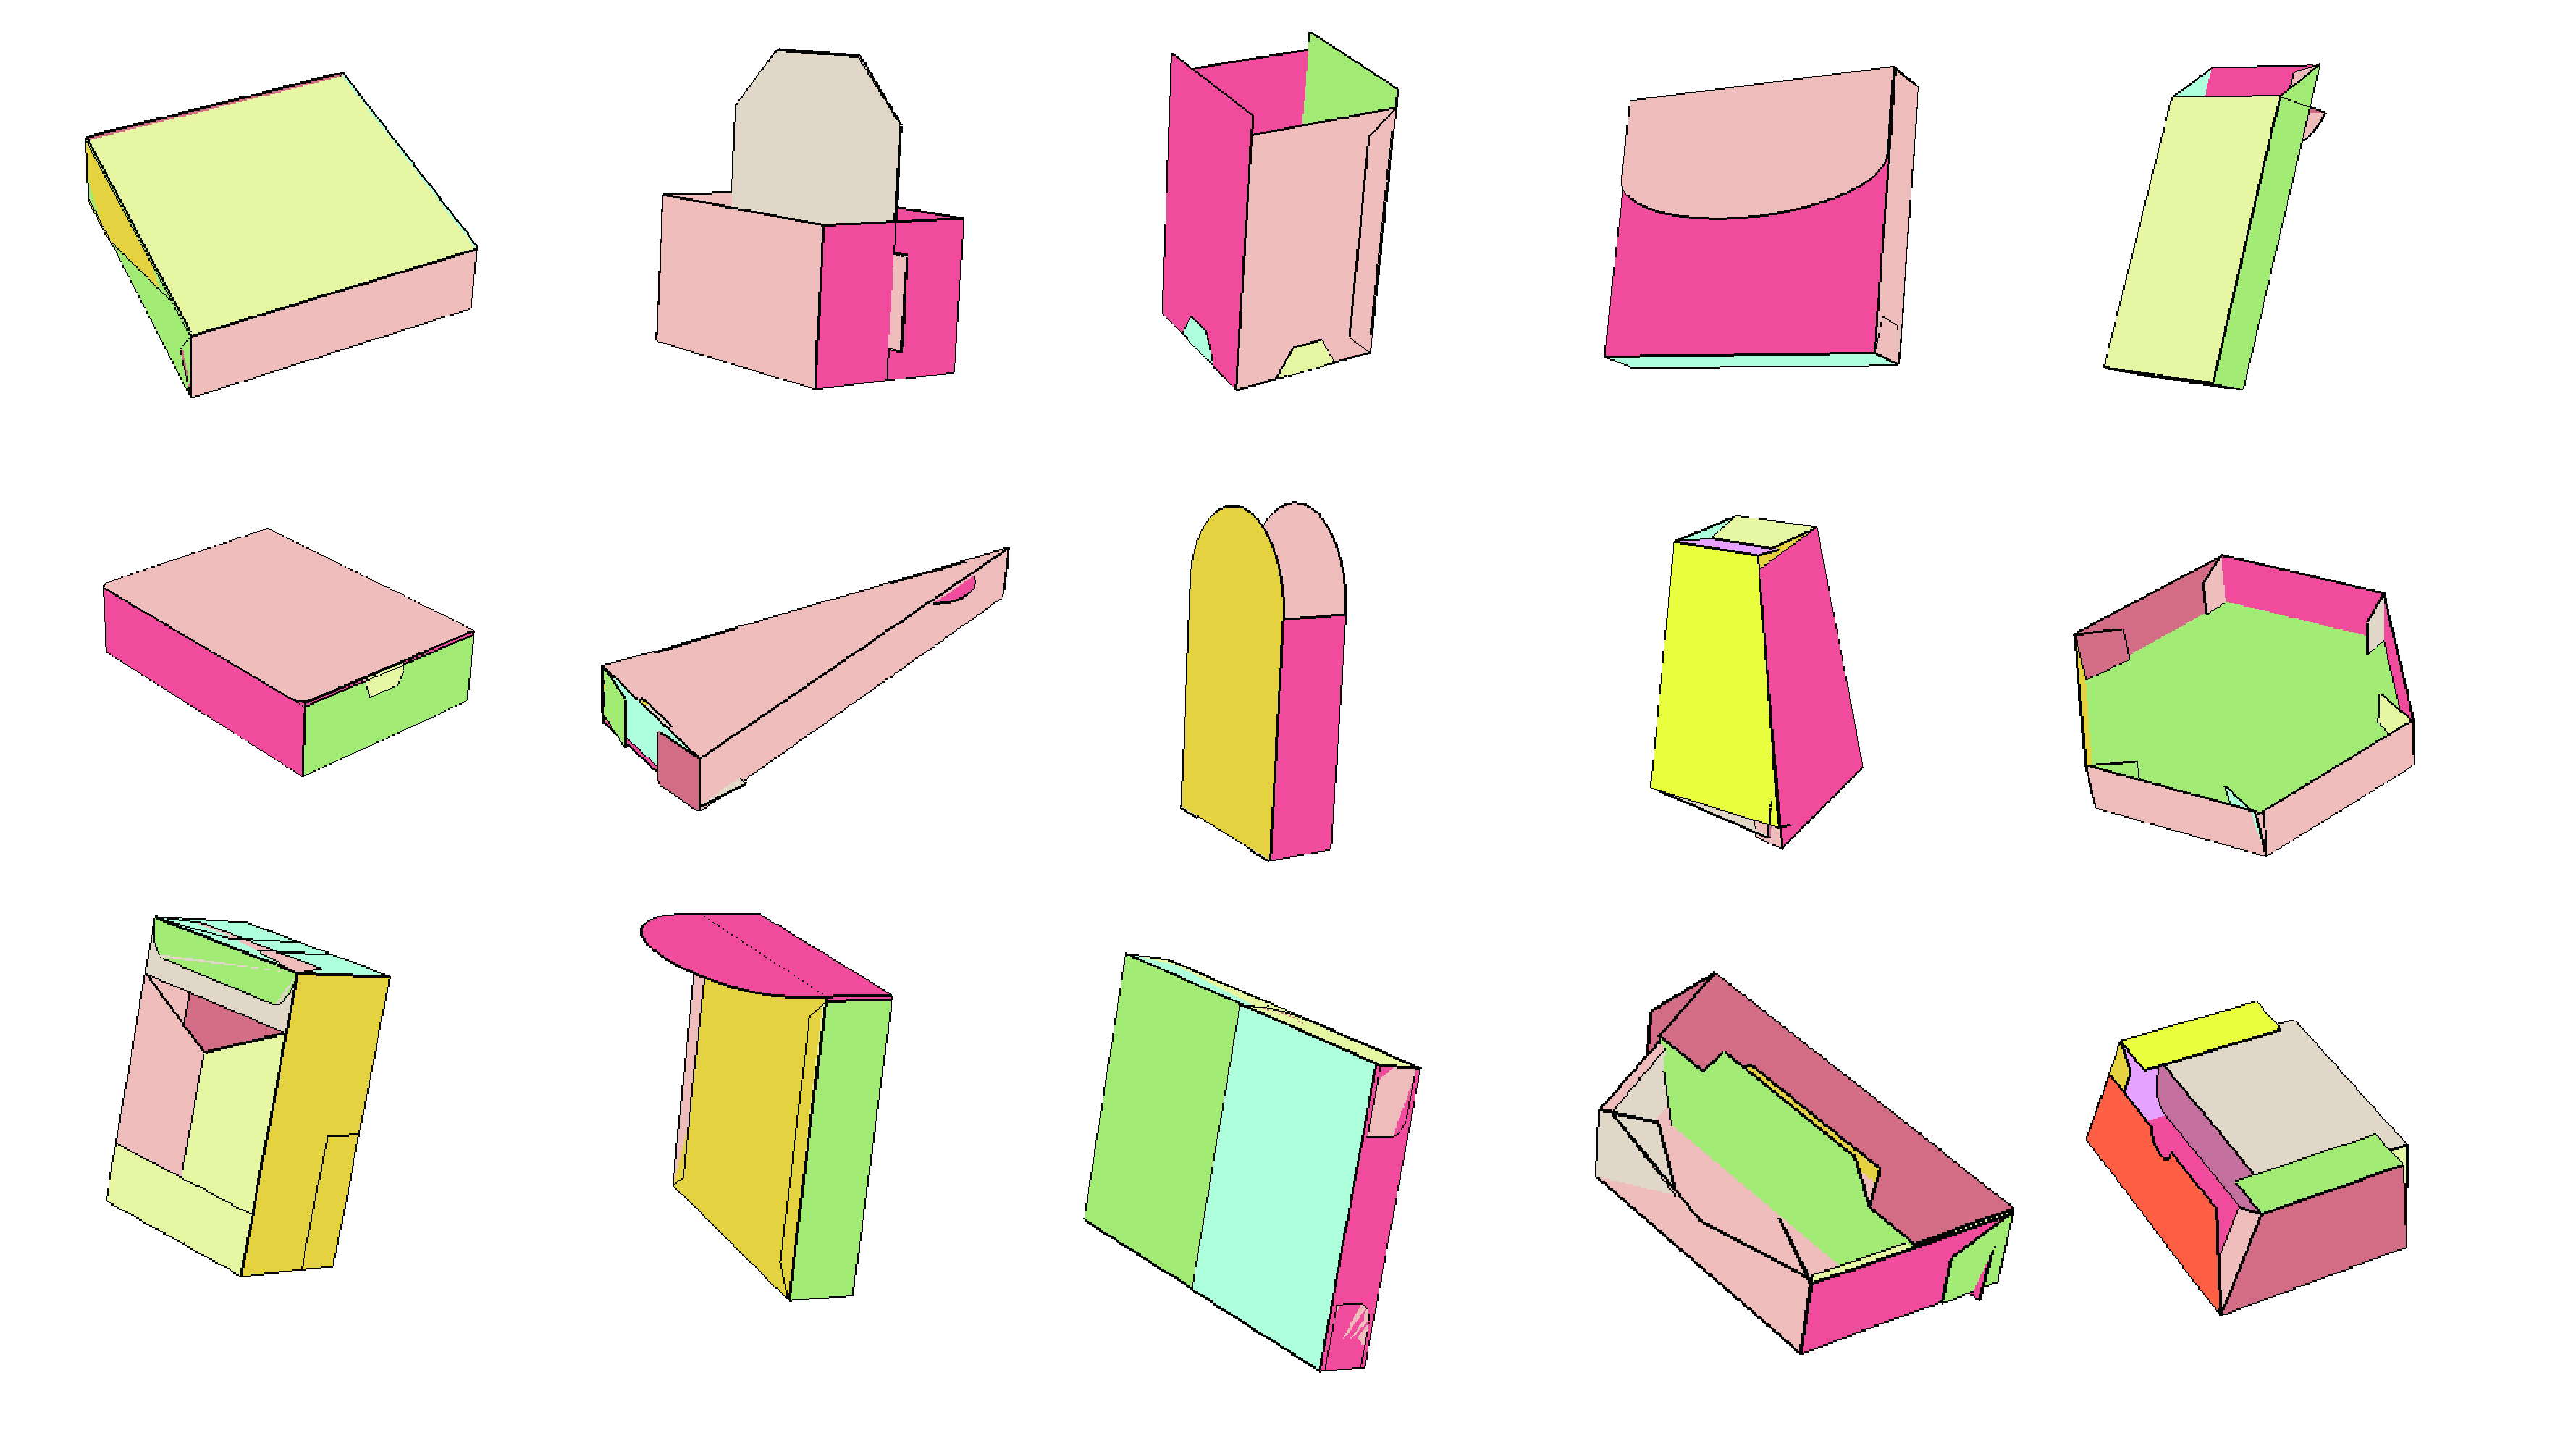
\includegraphics[width=0.9\textwidth]{images/initial2.jpg}
	\caption{15 different initialization results. Eight of them need not further refine. \cxj{show the input. point out which 8.}}
	\label{fig:initial}
\end{figure}

%%%%%%%%%%%%%%%%%%%%%%%%%%%%%%%%%%%%%%%%%%%%%%%%%%%%%%%%%%%%%%%%%%%%%

\subsection{Shape Constrain}
After initialization, there is still a need to refine the results that have not folded into pleasing results. The main idea is to prescribe the shape constrains by a set of vertices of the polymesh. Moreover, with the extra information acquired from user interaction, we can finally construct the ideal 3D realization compared to the ground truth. As you can see, the coordinate of vertices are chosen as our input instead of fold angles on edges, the reason is that constrains represented by vertices are simpler and more intuitive than angles, and we can implement the algorithm introduced by Bouaziz et al. easily~\cite{Bouaziz:2012:SSD:2346796.2346802}.

We now introduce the constrains used in our construction method:

\noindent
\textbf{Edge Constrain} For each edge $\{e_j\}_{j=1...M}$, we have its start point $\mathbf{v}_{js}$ and end point $\mathbf{v}_{jt}$, then we have 
\begin{equation}
||\mathbf{v}_{js} - \mathbf{v}_{jt}||^2 = ||\mathbf{\hat{v}}_{js} - \mathbf{\hat{v}}_{jt}||^2,
\label{equ:edge}
\end{equation}
to ensure that the length of each edge stays the same.

\noindent
\textbf{Coplane Constrain} For each plane $\{p_k\}_{k=1 \dots P}$ and its normal $\mathbf{n}_k$, each line connected by two points $\mathbf{v}_{ka}, \mathbf{v}_{kb}$ on the plane is perpendicular to the normal.
\begin{equation}
\mathbf{n}_k \cdot (\mathbf{v}_{ka} - \mathbf{v}_{kb}) = 0.
\label{equ:coplane}
\end{equation}

\noindent
\textbf{Plane Constrain} For each plane $\{p_k\}_{k=1 \dots P}$, the length of each line connected by two non-adjacent points $\mathbf{v}_{ka}, \mathbf{v}_{kb}$ on the plane remains the same, so that the shape of each plane keeps unchanged.
\begin{equation}
||\mathbf{v}_{ka} - \mathbf{v}_{kb}||^2 = ||\hat{\mathbf{v}}_{ka} - \hat{\mathbf{v}}_{kb}||^2.
\label{equ:plane}
\end{equation}

The information acquired from user interaction will add enough constrains to solve the optimization problem, and one of the interaction is to choose the right given suggestion including points needed to be merged together. As for the point information, the constrains can be written like:

\noindent
\textbf{Point Constrain} 
\begin{equation}
\mathbf{v}_p - \mathbf{v}_q = 0,
\label{equ:point}
\end{equation}
if these two points $\mathbf{v}_p$, $\mathbf{v}_q$ need to be moved into the same place.

When the above constrains still lead to an ill posed problem, a soft constrain will be introduced:

\noindent
\textbf{Irrelevant Point Constrain} Points $\{\mathbf{v}_i\}$ which are not in the same plane with $\mathbf{v}_p$ or $\mathbf{v}_q$, should be near the original location, and this constrain just take a light weight $w$, which is set 0.001 in our experiment. 
\begin{equation}
\mathbf{v}_i - \mathbf{\hat{v}}_i = 0.
\label{equ:irrelevant}
\end{equation}

Figure~\ref{fig:constrain} illustrates the necessity of basic three constrains.

\begin{figure}
	\centering
	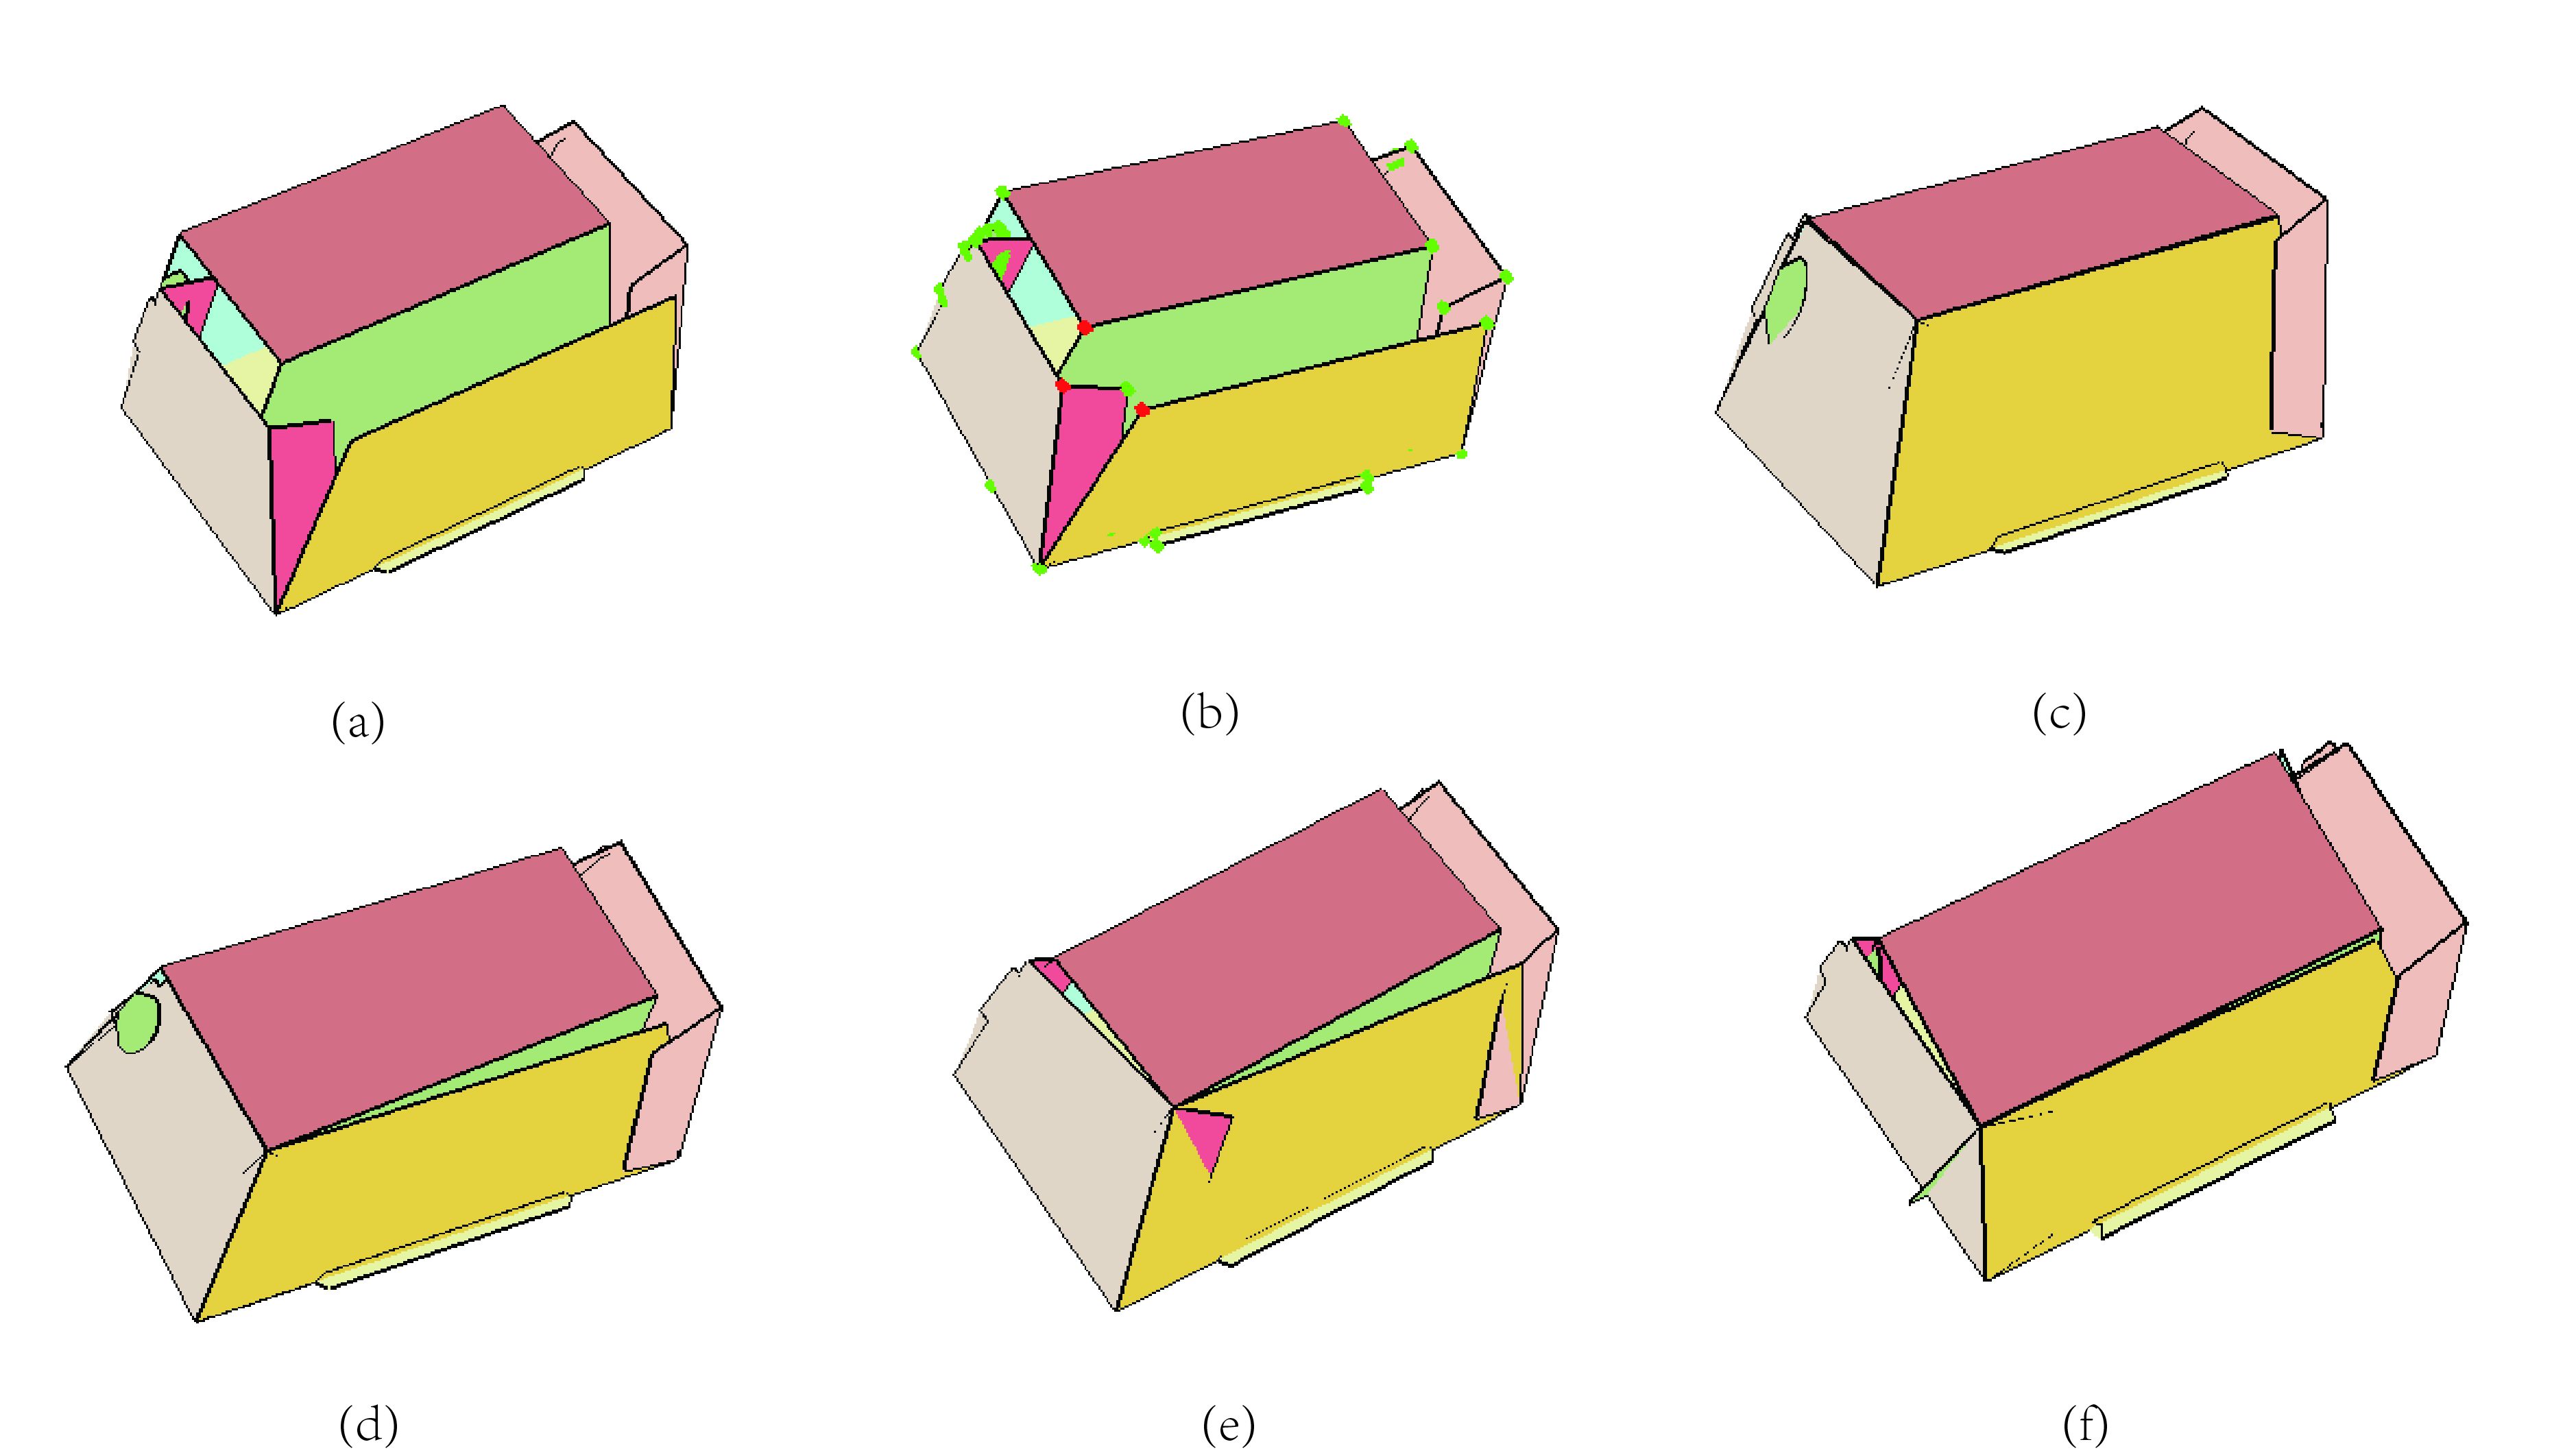
\includegraphics[width=0.9\textwidth]{images/constrain.jpg}
	\caption{Given an initial state~(a), by choosing three points marked in red~(b) that need to be relocated together, basic three shape constrains can lead to the optimization result~(c). The bottom three are the results optimized lack of edge constrain, coplane constrain and plane constrain separately, compared to~(c), the results can not keep the basic shape well.}
	\label{fig:constrain}
\end{figure}


\subsection{Aided Detection}

While the initial 3D model with simple angle folding provides a rough idea about the carton shape, our system could automatically detect a group of possible shape constraints to form the final 3D model, such as vertex merging, shape symmetry, and so on. 
%
These guiding operations are provided to the user at bottom of the user interface, for the user to quickly select and explore the carton shapes.

%
In order to asist users construct the final carton interactively, we also provide symmetry detection and merging points detection to improve the efficiency of constructing models .

\noindent
\textbf{merging points detection} Consider the initialization results can represent the ideal model partly, the disadjacent vertices that have one edge with same length can be regarded as targets that need to be located in the same place if their Euclidean distance is below a certain threshold.

\noindent
\textbf{symmetry detection} On account of the simplicity of the carton shape, the vertices that have same length set of incident edges can be regarded as symmetric pair. While users select vertices that need to be merged together, symmetry detection can reduce repetitive work by giving users suggestions of symmetric vertices.